\documentclass[output=paper]{LSP/langsci} 
\ChapterDOI{10.5281/zenodo.1090996}
\title{Aspects of a primacy of frame model of translation}
\author{Oliver Czulo
\affiliation{University of Leipzig}
}

\abstract{Frame Semantics and Construction Grammar are two highly interdependent cognitive linguistic theories which have been used in various ways to date to analyse and model translation. However, a unified model on how frames and constructions (are) operate(d on) and interact in translation, i.e. a translational perspective on and of frames and constructions, has not yet been fully developed. The model proposed in this paper is intended to narrow this gap. In drafting this model, I establish the principle of maximum frame comparability. I furthermore analyse factors which may lead to an override of this principle. From these analyses, I deduce research questions the investigation of which can benefit both translation studies as well as the theoretical frameworks Frame Semantics and Construction Grammar.}

\maketitle
\begin{document}

\section{Introduction}\label{czulo:sec:1}

Though we can contend that ``transferring'' ``meaning'' is the main objective of a translation, the wish to ``transfer'' this ``meaning'' in a precise and adequate fashion often collides with constraints e.g. on the forms we can use, or in other words the grammar of a language. This can be observed in the following example from the CroCo-corpus \citep{HansenSchirra2012Cross}:


\ea\label{czulo:ex:1}  Einzelheiten können Sie diesem Bericht entnehmen.\\
Details can you from-this report take.out \\
\glt Additional details are contained in this report.
\z
% \chapter[Einzelheiten können Sie diesem Bericht entnehmen. Lit.: `Details can you from{}-this report take{}-out'Additional details are contained in this report.]{Einzelheiten können Sie diesem Bericht entnehmen. \\
% Lit.: `Details can you from-this report take-out'\\
% Additional details are contained in this report.}

In the \ili{German} original, we have a \isi{construction}, a sentence initial direct object followed by the finite verb, which cannot usually be reproduced as such in English. There are various ways how to deal with this in translation \citep{HansenSchirra2008, Culo2016}, focussing on various aspects of the original. In this case, the translator decided to leave the \textit{details} in sentence-initial position, giving it a certain attention focus, similar to the \ili{German} original. As the sentence initial element in English usually is the subject, \textit{details} is shifted from the direct object to the subject grammatical function. With a new subject in the translated sentence, the main verb is accommodated accordingly, resulting in a different perspective and thus a slight shift in ``meaning'': While the \ili{German} original speaks of an action, somebody taking out something from a ``container'' (i.e. the \textit{report}), the English translation describes a state, i.e. something as being inside a ``container''. This shift leaves us with at least two questions: If meaning is central to translation, which factors can lead to shifts in ``meaning''? And how can we describe shifts in ``meaning'' in a systematic manner, making use not of prose but e.g. of abstract schemata?

``Meaning'' can involve various aspects. Without diving too deeply into any philosophical discussion on what ``meaning'' exactly entails, we can distinguish at least two aspects on a coarse level of abstraction: First, the information that is contained in an expression or its \textit{semantics}. This is comparable to the idea of the propositional act \citep{Searle1969}, which entails references to entities and predications on them. It is information expressible in abstract, schematic ways, but not the meaning as it is construed by an individual and enhanced with personal emotional, associative, aesthetic or other aspects. Second, the effects that we connect with the way we present the information, or in other words the \textit{function} of an expression. This is different from the intentions of a speaker/writer, which are not available to us unless shared with us (even though they can often be at least partially inferred), whereas the function of an expression, e.g. guiding attention focus towards a certain element within a larger \isi{construction}, is collective knowledge. In the above example, two aspects of ``meaning'' collide: The attention focus that is put on the sentence initial element by the \ili{German} sentence \isi{construction}, the perspective on the information and the actions around it resp. its state, and last but not least the formal grammatical make-up of the sentence such as what the subject of the sentence is. The problem in example \ref{czulo:ex:1} is that not all three aspects, form, function and semantics can be fully rendered the same way at the same time in one message in the \isi{target language}.

The translation aspects in focus in this paper are thus the operations on form and semantics during a translation, with a certain function in mind, and the interaction of these aspects.

\newpage 
In this paper, I present the draft of a model of translation which focuses on these aspects of translation and aims at an integrated view of the three dimensions form, function and semantics. It aims at describing how these dimensions may manifest in similarities and differences between original and translation product, with occasional reference to which role processual factors may play.

In order to model the linguistic aspects of translation along these three dimensions, I make use of Construction Grammar (henceforth CxG, cf. e.g. \citealt{Fillmore1985Syntactic}; \citealt{Goldberg1995})\footnote{The references cited here refer to different incarnations of Construction Grammar, but the principles of CxG referred to herein are shared by these varieties.} for more form-oriented aspects and Frame Semantics (henceforth FS, \citealt{Fillmore1982}; \citealt{Fillmore1985Frames}) for semantics-oriented aspects. Function manifests as the choice of certain formal or semantic aspects over others. I have chosen CxG and FS because these theories do not solely rely on studying a system of signs or constructs, but they also assume that background knowledge, including personal and cultural backgrounds and beliefs as well as world knowledge, is directly involved in producing or understanding linguistic expressions. According to these theories, links between forms and meanings are conventionalised, and these conventions can be learned, extended and changed. In their basic assumptions, CxG and FS are thus highly compatible both with the aim of this paper and a functional-cognitive view on translation serving as the backdrop of the model proposed in this paper.

In this model, I assume that the semantics of an expression is what by default makes up for the key considerations in translation. As the semantics is represented by means of \isi{frame} descriptions, it is called the \textit{primacy of frame} model. By saying ``primacy of \isi{frame}'', I do not mean to imply that semantic information is processed first or necessarily processed at all on a neurocognitive level; but in a cloud of features representing functional, formal and semantic aspects, by default semantic aspects should receive most consideration. In developing this model in the following sections, I will also present cases in which, I believe, formal or functional considerations override certain semantic ones, rounding off a model in which, though we can assume the various dimensions to be somewhat structured internally, no dimension is immutable and none is absolute.

The model drafted here does not only address translation settings involving one lonely translator in their quiet chamber. The methods of analysis applied here rest on principles laid out by CxG and FS which I assume collectives (can) share. The model should thus just as well cover translations that were made by a crowd or revised at a later stage.

\newpage 
While I will mainly be using CxG and FS for the analyses in this paper, this model does not intend to be an island theory. It is quite clear to me that CxG and FS analyses will not suffice to explain each and every translation phenomenon. The two cognitive linguistic theories used here are, however, compatible with a number of other theories such as the \isi{metaphor} theory by \citet{Lakoff1980, Lakoff1999} or mental spaces theory by \citet{Fauconnier2002} which can serve as further explanatory devices. 

I am also aware that some of what will be said here may be reminiscent of and hopefully much of it compatible with what has been said in other places in cognitive (translation) studies, e.g. on the cognitive basis of translation phenomena \citep{Halverson2003}, linguistic theory and how it can be modelled by means of networks, e.g. Word Grammar \citep{Hudson2007} and an extensive body of process-based and neurocognitive investigations into translation (cf. \citealt{Gopferich2008, Aitchison2012} for an overview). The model drafted here simply represents a FS and CxG perspective. In later stages, it should be aligned with findings from the fields cited above. In this paper, I will focus on the aspects of a frame-and-constructions analysis and explanation as I envision it and on highlighting which benefits I expect from adding FS and CxG to the mix (\sectref{czulo:sec:3}). I will also lay out further principles beyond those stated above for a primacy of \isi{frame} model, deducing from them further research questions (\sectref{czulo:sec:4}).

In drafting this model, I will refer to empirical findings of a number of researchers (including myself) and will attempt to come up with a coherent model. These findings do not only involve findings from corpus studies, but to a lesser extent also from \isi{translation process} and neurocognitive studies. It needs to be pointed out, though, that this model is rather a \textit{mental} model of translation, as opposed to a \textit{neurocognitive} model; i.e. it deals with a higher level of abstraction of operations, both conscious and subconscious. Some statements made here may run counter to findings from neurocognitive studies. I will, however, leave the resolution of potential contradictions to future research.

\section{Frames, constructions and translation}\label{czulo:sec:2}
\largerpage
In recent years, the cognitive paradigm has been on the rise in translation studies, as witnessed by a growing number of events and publications on the topic. As the informed reader will know, this not a completely new topic, though. It was already in the 1980s that, for instance, \citet{Krings1986Was} used Think-Aloud-Protocols to look into what is going on ``inside the translators' minds''. Recent advances in technology have opened new windows into the translators' minds: By means of key logs, eye tracking protocols, brain imaging techniques etc. we can look not only into conscious verbalisations, but also into unconscious operations and strategies during the \isi{translation process}.

The idea of using FS to model a product-oriented perspective on what ``goes on'' inside the translators' minds is not a new one, as we will see in the following. More recently, CxG has also been playing a role in Translation Studies. In the following subsections, I will first give a brief introduction into FS and CxG and will then present some approaches which involve at least one of the two theories and are relevant for this line of work. 

\subsection{Frame semantics and Construction grammar}\label{czulo:sec:2.1}

Frame semantics and \isi{construction} grammar both originate from Charles Fillmore's work. His valence theory-based Case Grammar \citep{Fillmore1968} soon evolved into a theory of a semantics of understanding \citep{Fillmore1985Frames}. While \isi{frame} semantics focuses on the semantic side of language, Construction Grammar \citep{Fillmore1985Syntactic} deals with the grammatical side. CxG has seen adoption by many, resulting in various incarnations of CxG. In this paper, I will not position myself in favour of any of those incarnations, but will stick to the basic tenets shared by most if not all theories belonging to the CxG family. \\

\noindent \textsc{Frame semantics} is a semantic theory of understanding: In his \isi{frame} semantic theory, Fillmore highlights the importance of background knowledge for the interpretation of linguistic expressions and thus distances it from purely truth-semantic theories. A \isi{frame} is defined as a:

\begin{quote}
... system of concepts related in such a way that to understand any one concept it is necessary to understand the entire system; introducing any one concept results in all of them becoming available. \hfill --- \citet{Petruck1996} 
\end{quote}

\noindent The theory of \isi{frame} semantics is closely entrenched in a linguistic paradigm. While FS in many ways is a theory of the system of concepts prevalent in a culture (or, more generally, a collective of speakers), it also captures the relation between linguistic material and mental concepts. A \isi{frame} is \textit{evoked} by means of linguistic expressions, and by this evocation our background knowledge is activated and helps us interpret an expression. One of the most popular examples to describe this is by means of the \textsc{Commercial\_transaction} \isi{frame}. In this \isi{frame}, a \textsc{Buyer} and a \textsc{Seller} are involved in a transfer of \textsc{Goods} in exchange for \textsc{Money}. This \isi{frame} can be perspectivised in various ways: In the \textsc{Commerce\_buy} scenario, the focus is on the \textsc{Buyer}, in the \textsc{Commerce\_sell} scenario on the \textsc{Seller}. But the fact that the \isi{frame} is linked to the evoking elements such as \textit{buy}, \textit{purchase}, \textit{sell}, \textit{price}, etc. and that the \isi{frame} as a whole is activated in the process of interpretation allows us to fully understand partial instantiations of a \isi{frame}. So when we read/hear a sentence like 
\ea\label{czulo:ex:2}
Jane sold her house.
\z
we understand that it was sold to someone and for a certain amount of money, even though this is not explicitly mentioned.

This example highlights an aspect of the theory which is central to it -- and interesting with respect to translation: the various different realisation of a \textsc{Commercial\_transaction} are instances of different perspectives on events. This notion of perspective is an important one in translation: it is not rare to find shifts in perspectives in translations, as demonstrated by the following well known example from \citet[104]{Vinay1995}: 
\ea\label{czulo:ex:3}
\gll Blériot traversa la Manche par avion. \\
 Blériot traversed the channel by plane \\
\glt Blériot flew across the channel.
\z
While in the \ili{French} version it is the direction of motion that is encoded in the verb, the English version realises the manner of motion in this place. The two different frames instantiated here can easily be related to each other, coming from the same domain. Also, this difference in how motion events are usually encoded in \ili{Romance} and Germanic languages is well documented (cf. e.g. \citealt{Talmy2000, Slobin2004}). One question of course is to which extent such shifts in perspective can be described and explained by means of \isi{frame} semantic analysis. This question will be addressed in \sectref{czulo:sec:2.2}.

FrameNet \citep{Fillmore2003} contains a list of frames together with the linguistic expressions they are connected to based on corpus data. Each \isi{frame} entry gives a definition as well as a list of core and peripheral \isi{frame} elements. For lexicalised frames, a list of lexical units which evoke the \isi{frame} is given, and for many lexical units, corpus examples and the annotation scheme can be viewed. Frames do not stand just for themselves, but are also connected to each other via frame-to-\isi{frame} relations. The frames \textsc{Filling} and \textsc{Fullness}, for instance, are connected via the \textit{inchoative of-relation}, where \textsc{Filling} is inchoative of \textsc{Fullness}. Other relations currently defined include such relations as \textit{inheritance}, \textit{precedence} or \textit{causation}. FrameNets exist in various other languages, with differences in coverage, e.g. for \ili{German} (named SALSA, \citealt{Burchardt2006}), for \ili{Japanese} \citep{Ohara2004} or \ili{Spanish} \citep{Subirats2003}.\\

\noindent \textsc{Construction grammar} has a variety of incarnations (e.g. 
\citealt{Fillmore1985Syntactic}; \citealt{Fillmore2012};
\citealt{Goldberg1995,Goldberg2006}%
), but all of them based on a set of compatible definitions and assumptions (cf. \citealt{Stefanowitsch2007} for an overview). Most notably, CxG does not assume a strict division between lexicon and grammar, but rather a continuum. A \isi{construction} is defined as a pairing of form and meaning; the concept of form comprises the whole range from morphemes to lexemes to phrasemes to grammatical patterns and even textual patterns. For instance, the \textit{Caused Motion} \isi{construction} \citep[3, 9f.]{Goldberg1995} is realised by the pattern \textit{Subject-Verb-Object1-Oblique}, as in the following example:

\ea\label{czulo:ex:4}
Pat sneezed the napkin off the table. 
\z
Though \textit{sneeze} is not usually thought of as a transitive verb, we understand the caused motion aspect when it is used in within the grammatical pattern associated with the \isi{construction}. The form-meaning pairing is conventionalised and the frequency of occurrence is crucial both for acquiring as well as entrenching a \isi{construction} as such.

The Berkeley Constructicon \citep{Fillmore2012}, an extension of FrameNet, contains a list of constructions with the definition of their grammatical pattern, the list of the \isi{construction} elements and an informal description of their semantic and pragmatic properties. This Constructicon, which lists English constructions, is used as blueprint and as source for contrastive studies for Constructicons in other languages such as \ili{Swedish} \citep{Skoldberg2013} or \ili{German} \citep{Boas2013}.

\subsection{Applying frames and construction to translation or the analysis of translation}\label{czulo:sec:2.2}

There have been a number of studies and approaches to studying translation by means of FS and/or CxG; the list of those presented in the following is certainly more than incomplete. What they lack, however, is a unified, consistent model not of how FS and CxG may serve as linguistic theories for the study of translation, but of how they may serve as \textit{translational} theories (though, of course, with a linguistic perspective). An underlying, common model should connect these studies, which sometimes give a very broad idea of how to apply FS and CxG in a translational perspective, and sometimes focus on very specific phenomena, not taking the great big whole into account. Based on the following coarse overview of relevant studies and approaches, I will identify some of the benefits I expect from taking a translation perspective on frames and constructions in \sectref{czulo:sec:3}, where I will also identify the research questions which are connected to a unifying model, the primacy of \isi{frame} model, presented in \sectref{czulo:sec:4}.

Vannerem \& Snell-Hornby's \citeyearpar{Vannerem1986} approach already contains some of the ingredients of a primacy of frame-model. According to them, there can be three ways of translating: By means of a \textit{scene-to-scene}, \textit{scene-to-frame} or a \textit{frame-to-frame} transfer. Their theory is based on earlier versions of \isi{frame} semantics, then still named \textit{scenes-and-frames} semantics, where the scene roughly corresponds to a \isi{frame} and the \isi{frame} roughly to a (phrasal or sentential) \isi{construction}. Vannerem and Snell Hornby's model is based, in current terminology, on the following key observation: If the \isi{frame} in source and \isi{target language} are equivalent for the given context, the transfer is simply a matter of finding the right \isi{construction}(s) in the \isi{target language}, resulting in a construction-to-\isi{construction} transfer. Sometimes, however, adaptions need to be made in terms of the semantics (the \isi{frame}, in our current terminology), but the authors give a few examples of adaptions that can be made.

\citet{Kussmaul2000} discusses a number of kinds of adaptions on the semantic level that may occur in translation. He cites various cognitive theories such as script theory, lateral thinking and \isi{frame} semantics, and integrates them into a four-phase approach to translating. He demonstrates how, by means of using our knowledge of frames, we can find translation solutions that go beyond an exact reproduction of the original. He discusses the translation of a line from the Musical \textit{Cats} (ibid.: 158f.), where, given the constraints of metrics, an exact translation is not always possible:

\ea\label{czulo:ex:5}
\gll Als man täglich von ihm in der Zeitung gelesen \\
When one daily of him in the newspapers read. \\
\glt Though his name was very famous, he says, in his time
\z
% \chapter[``Though his name was very famous, he says, in his time''``Als man täglich von ihm in der Zeitung gelesen''Lit.: `When one daily of him in the newspapers read.']{``Though his name was very famous, he says, in his time''\\
% ``Als man täglich von ihm in der Zeitung gelesen''\\
% Lit.: `When one daily of him in the newspapers read.'}

Being famous activates frames in which it is defined that fame comes with regularly being on TV or in the newspapers. This is thus a case of activating parts of a larger \isi{frame} within a domain. Kußmaul's approach offers a number of insights into how different frames may be connected and how their connections can be exploited.

\largerpage
The foci of the two models by Vannerem/Snell-Hornby and Kußmaul are somewhat different: Vannerem and Snell-Hornby present a more general approach on how frames and constructions serve as points of orientation in translation, with various types of replacement operations (e.g., in their terminology, frames for scenes, frames for frames). Kußmaul shows how the background knowledge connected to a \isi{frame} can be exploited to choose different perspectives in translation. Neither of the two approaches is spelled out in such a way, though, that types of permissible links are investigated and they are somewhat underspecified as to which factors (generally) lead to which sort of shift.

\citet{Pado2005} report on a finding with regard to systematic differences between English and \ili{German} in framing causation for events like changing a position on a scale. They survey a small English-\ili{German} sample from Europarl \citep{Koehn2005} with the translation pair \textit{increase} -- \textit{höher} `higher'. When a Cause or Agent is present with \textit{increase}, the lexeme is associated with the \textsc{Cause\_change\_of\_position\_on\_scale} \isi{frame} (CCPOS), else with the \textsc{Change\_of\_position\_on\_scale} \isi{frame} (CPOS). The \ili{German} adjective \textit{höher} can only instantiate the \textsc{CPOS} \isi{frame} (in this particular meaning); the causation aspect is then expressed by a second \isi{frame} in the sentence, such as in the following sentence pair (cf. \citealt{Pado2005} \isi{frame} evoking elements in caps, \isi{frame} elements in brackets):  

\ea\label{czulo:ex:6}
wenngleich [der Welthandel]\textsc{\textsubscript{Cause}} [einen HÖHEREN\textsubscript{CPOS} [Wohlstand]\textsc{\textsubscript{Item}}]\textsc{\textsubscript{Effect}} ZUR FOLGE HAT\textsubscript{CAUSATION}\\
\medskip

though [world trade]\textsc{\textsubscript{Cause}} can of course INCREASE\textsubscript{CCPOS} [prosperity]\textsc{\textsubscript{Item}}\textsc{\textsubscript{} } \\
\glt `[\ldots ] even if world trade has higher prosperity as result'
\z
% \chapter{EN:  \ldots though [world trade]\textsc{\textsubscript{Cause}} can of course INCREASE\textsubscript{CCPOS} [prosperity]\textsc{\textsubscript{Item}}\textsc{\textsubscript{} }}
% \label{bkm:Ref438069244}\chapter{DE:  \ldots wenngleich [der Welthandel]\textsc{\textsubscript{Cause}} [einen HÖHEREN\textsubscript{CPOS} [Wohlstand]\textsc{\textsubscript{Item}}]\textsc{\textsubscript{Effect}} ZUR FOLGE HAT\textsubscript{CAUSATION}\\
% Lit.: `[\ldots ] even if world trade has higher prosperity as result'}

The lexical units \textit{increase}, \textit{höher} `higher' and \textit{zur Folge hat} `have as a result' evoke the \textsc{CCPOS}, the \textsc{CPOS} and the \textsc{Causation} \isi{frame} respectively (marked by underlining in the example). In the \ili{German} version, the inchoative \textsc{CPOS} \isi{frame} is embedded in the \textsc{Causation} \isi{frame}, and together they convey the meaning which is conflated in the \textsc{Ccpos} \isi{frame} in the English version.\footnote{I speak of ``versions'' here because it is not clear from \citet{Pado2005}, whether the examples were checked for the status ``original'' or ``translation''; nevertheless, the relation described here seems to hold irrespective of the original vs. translation status in their sample.} The authors note that in their data, the adjective \textit{höher} is only used in the inchoative meaning, which results in the consistently observed  pattern of two-to-one \isi{frame} matches between \ili{German} and English versions.

\citet{Serbina2013} studies constructional shifts when translating the basic \textit{Subject-Verb-Object} \isi{construction} in English into \ili{German}. She finds that there is a tendency for shifts (though not a strictly significant one) when the subject is filled with an inanimate entity, something that has been described in the contrastive linguistic literature before (cf. e.g. \citealt{Hawkins1986, Konig2009}), as illustrated by examples such as the following \citealt[108]{Konig2009}):

\ea\label{czulo:ex:7}
\gll Mit dieser Werbung werden wir viel Hundefutter verkaufen. \\
With this advert will we much dog-food sell \\
\glt `This advert will sell us a lot of dog food.'
\z
% \chapter[This advert will sell us a lot of dog food.Mit dieser Werbung werden wir viel Hundefutter verkaufen. Lit.: `With this advert will we much dog food sell']{This advert will sell us a lot of dog food.\\
% Mit dieser Werbung werden wir viel Hundefutter verkaufen. \\
% Lit.: `With this advert will we much dog food sell'}

Serbina finds a tendency for shifts in cases in which the English original has an unagentive subject. According to her evaluation scheme -- in which she does not only distinguish between agentive and unagentive, but between human, animate and inanimate -- the effect is only weakly significant, though.

The studies by Padó and Erk and by Serbina investigate specific factors for \isi{frame} or \isi{construction} shifts in translation. Their studies can serve as blueprints for further studies, and their findings can be well integrated into a model studying factors for such shifts.

\citet{Rojo2013} look at constructions from a process-based perspective. They focus on a case of \textit{constructional mismatch}: The English resultative \isi{construction} has no counterpart in \ili{Spanish}, unlike the English predicative \isi{construction}. In their experiment, they asked their subjects to translate sentences of which some were given in the predicative variant such as \textit{She hammered the metal until it was flat} and the resultative variant \textit{She hammered the metal flat}. The authors find that translating the resultative variant into \ili{Spanish} took longer and resulted in more fixations than for the predicative variant, underlining the relevance of the concept of a \isi{construction} in the \isi{translation process} and building a bridge from product-oriented linguistic theory to process-oriented cognitive studies.

In \citet{Culo2013}, I combine \isi{construction} analysis and \isi{frame} analysis to study shifts in form and meaning of a translation which I hypothesise to be induced by a constructional mismatch, such as the sentence initial direct object followed by a verb in \ili{German}. An example of this is the following sentence pair:

\ea\label{czulo:ex:8}
\gll Handlungsbedarf wird ES auch weiterhin GEBEN\textsubscript{EXISTENCE} . \\
Need-for-action will it also furthermore give \\
\glt More changes will TAKE PLACE\textsubscript{EVENT} in the future .
\z
% \chapter{Handlungsbedarf wird ES auch weiterhin GEBEN\textsubscript{EXISTENCE} .\\
% Lit.: `Need-for-action will it also furthermore give'\\
% More changes will TAKE PLACE\textsubscript{EVENT} in the future .}
As I report in \citet{Culo2016}, there are various strategies to deal with this. The simplest would be to just switch the order of subject and object, losing the focus on the direct object. In \REF{czulo:ex:8}, the translator decided, it seems, to mimic the information structure of the original sentence, but by shifting the element which was a direct object in \ili{German} into the subject in English, the main verb of the sentence needs to be accommodated. This results in a \isi{frame} shift between the sentences: While the \ili{German} original speaks of the \textsc{Existence} of a need for change, the English version describes the \textsc{Event} of a change happening in the future. Despite this shift in semantics\footnote{And leaving out the question of whether the context licenses this shift.}, we can still relate the two sentences to each other in terms of ``semantic similarity'' and model this relation by means of exploiting frame-to-\isi{frame} relations as proposed by \citet{Ellsworth2006} and demonstrated in \figref{czulo:fig:1}.


\begin{figure}
    \resizebox{.5\textwidth}{!}{
    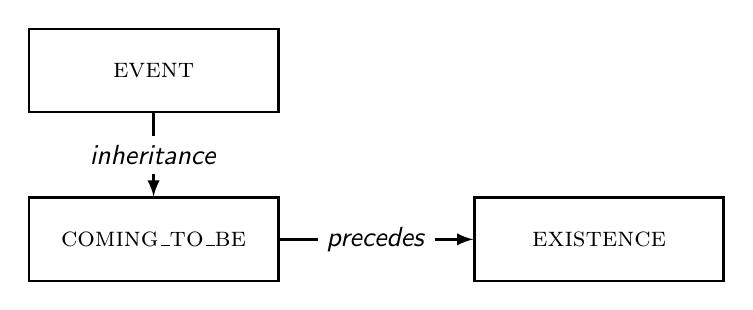
\begin{tikzpicture}
        \usetikzlibrary{shapes,arrows,positioning}
    % Define Styles
        \tikzstyle{block} = [rectangle, draw, fill=white, text centered, minimum height=3em, minimum width = 9em, line width = 0.1em]
        \tikzstyle{line} = [draw, -latex, line width=0.1em]
    % Place nodes
        \node [block] (event) {\textsc{event}};
        \node [block, below = 3em of event] (coming) {\textsc{coming\_to\_be}};
        \node [block, right = 7em of coming] (existence) {\textsc{existence}};
    % Edges
        \draw[line] (event) -- (coming) node [midway, fill=white] {\sffamily\textit{inheritance}};
        \draw[line] (coming) -- (existence) node [midway, fill=white] {\sffamily\textit{precedes}};
    \end{tikzpicture}
    }
 %
\includegraphics[width=.5\textwidth]{figures/czulo/figure1.png}
 \caption{Frame-to-frame relations connecting the frames \textsc{Existence} and \textsc{Event}}
 \label{czulo:fig:1}
\end{figure}

The \textsc{Existence} \isi{frame} is preceded by the \textsc{Coming\_to\_be} \isi{frame} which, in turn, inherits from the \textsc{Event} \isi{frame}. The frames \textsc{Existence} and \textsc{Event} are thus closely related and we can state that the two sentences in (\ref{czulo:ex:8}) are semantically similar, something that we would expect of an original and a translation.

The cross-lingual application of such frame-to-\isi{frame} relations opens up more questions than it answers. The English \isi{frame} hierarchy can be well exploited where regions of the \isi{frame} hierarchy are structured in the same way. It is not clear yet, though, how to proceed in cases where regions of the \isi{frame} hierarchies for two languages are divergent, such as for the legal domain between \ili{Brazilian Portuguese} and American English \citep{Bertoldi2012}. Also, it is not yet clear how many steps through the \isi{frame} hierarchy we can take and still plausibly claim ``semantic similarity''. Nevertheless, this study exemplifies how to take an integrated perspective on both form and semantics, with function playing a key role in the choice of formal and semantic aspects.

\section{Frames and Constructions within a cognitive translation paradigm}\label{czulo:sec:3}

In the following I list the expected positive outcomes of using FS and CxG as basis for the primacy of frame-model, and I will also address cases in which FS and CxG benefit from testing and application within the primacy of \isi{frame} model.

\subsection{FrameNet and the Constructicon as resources}\label{czulo:sec:3.1}

One thing that both FS and CxG have to offer is that, through projects such as Frame Net and the Berkeley Constructicon, there is already an existing inventory of categories for \isi{frame} semantic and constructional units. Moreover, the English versions of these inventories have served as blueprints for similar projects in several other languages, among them SALSA as \ili{German} version of FrameNet \citep{Burchardt2006}, \ili{Spanish} FrameNet \citep{Subirats2003}, or the Berkeley Constructicon \citep{Fillmore2012}. These kinds of ``dictionaries'' are a treasure, certainly not only, but also for the study of various areas in Translation Studies such as semantic similarity, interaction of conceptual systems or grammatical conventions. Their inventories would need extension in coverage especially their non-English versions, to make them useful for a broad range of research questions, but this is, of course, a matter in which FS and CxG could go hand in hand with Translation Studies. 

As shown in the above-cited studies for translational purposes as well as for other, e.g. contrastive purposes (cf. \citealt{Boas2010}), FS and CxG annotation and analysis can serve well as a starting point for comparisons. At the same time, translational and contrastive studies may help uncover semantic and functional aspects that remain somewhat obscure in purely monolingual study settings. Consider, for instance, the following sentence pair and its frame-semantic annotation (CroCo-Corpus, \citealt{HansenSchirra2012Cross}, text pair G2E\_POPSCI\_007):

\ea\label{czulo:ex:9}
\gll [Besondere Probleme]\textsc{\textsubscript{Effect}} HAT\textsubscript{CAUSATION} man [MIT sadistischen und masochistischen Patienten] \\
Special problems has one with sadistic and masochistic patients \\
\glt [Sadism and masochism]\textsc{\textsubscript{Cause}} RAISE\textsubscript{CAUSATION} [special problems]\textsc{\textsubscript{Effect}} .
\z
% \chapter{[Besondere Probleme]\textsc{\textsubscript{Effect}} HAT\textsubscript{CAUSATION} man [MIT sadistischen und masochistischen Patienten]\textsc{\textsubscript{Cause}} .\\
% Lit. `Special problems has one with sadistic and masochistic patients'\\
% [Sadism and masochism]\textsc{\textsubscript{Cause}} RAISE\textsubscript{CAUSATION} [special problems]\textsc{\textsubscript{Effect}} .}

There are (at least) two notable observations to be made in this sentence pair. The first is on the grammatical level: The direct object \textit{Besondere Probleme} remains a direct object in the English version, whereas \textit{Sadism and masochism} shifts from a prepositional object to a subject in the English version (let us disregard the deletion of \textit{Patienten} for the time being). This may be due to a constructional mismatch: While \ili{German} easily allows the direct object in sentence initial position, it is rather unusual for English (cf. e.g. \citealt{Hawkins1986, Konig2009}). The other interesting observation to be made is the decision the translator made by translating the \ili{German} \textit{haben} `have' into the causative \textit{raise}. But does the \ili{German} \textit{haben} indeed have the standard reading of possession here? I would argue against it. A second look reveals that the translator might actually have had the \isi{construction} \textit{X haben mit Y} in mind. In \ili{German}, there are a few expressions like \textit{Probleme haben mit Y}, \textit{Ärger haben mit Y} etc. in which Y is an entity causing \textit{Probleme} or \textit{Ärger} `trouble'. However, this causative reading at the same time depends very much on the filler of X: In a phrase like \textit{Erfahrung haben mit Y} `have experience with Y', it seems somewhat debatable whether one would think of Y ``causing'' the experience. The \isi{construction} certainly begs a deeper investigation, but this shall suffice for the purpose of illustration: the causative reading of the \ili{German} sentence in (\ref{czulo:ex:9}) is only strengthened by the opposition of original and translation and by what one might call an expert decision. If we think of translators as expert communicators in context (both in a specifically linguistic and in general in a cultural context), then translation decisions like the one in (\ref{czulo:ex:9}) are an excellent source for extending FrameNet and the Constructicon. This example proves that developing the primacy of \isi{frame} model may benefit practical as well as theoretical aspects of FS and CxG.

\subsection{Frames and Constructions as multi-level description devices}\label{czulo:sec:3.2}

FS and CxG work on multiple levels of language. In fact, CxG does not assume the strict division between lexicon and grammar, defining a continuum of constructions through all levels of grammatical analyses, including morphemes, words and phrasal patterns (cf. e.g. \citealt[5]{Goldberg2006}). Also, grammatical patterns can carry ``meaning'' just as lexical units do; this ``meaning'' may be of the functional or the semantic type. The two theories are thus interconnected beyond matters of representation \citep[7]{Petruck1996}. It is this interconnectedness which facilitates an integrated analysis of the interplay of form, function and semantics in translation.

This interconnectedness and the principles established by the primacy of \isi{frame} model may also help push the boundaries of theory in other translation-related research, such as neuro-cognitive and process-based research. As \citetv{Oster} notes, many of the models for word processing in psycholinguistics are defined on the basis of word level. Assuming that words are constructions on equal footing with lower- and higher-level constructions, her network model of the lexicon can be easily extended to model e.g. how phrase patterns are connected and accessed in translation.

\subsection{Frames and Constructions as collective organisational schemata}\label{czulo:sec:3.3}

As \citet{Busse2012} notes, the question of whether frames relate to conceptual structures of an individual or a group, has been mostly left undiscussed. I argue that frames as they are defined in FrameNet are generalised abstract schemata of concepts shared by a collective. The definitions in FrameNet describe frames in a way in which they can be understood by most, if not all, members of the respective (sub)culture. This, however, does not exclude the fact that each \isi{frame} will receive a very individual ``instantiation'' in a speaker's mind.

Let us imagine a \textsc{Being\_at\_war{}}-\isi{frame} and a situation in which two parties are at war: The roles and relations described in a FrameNet lexicon will be recognizable by both parties, that there is a \textsc{War\_cause}, that there are \textsc{Warriors} and \textsc{Fight\_events}, as well as  \textsc{Civilians} involved/affected. Also, there will probably be a causer of the war, potentially called the \textsc{Attacker}. However, members from the different sides of the party will not necessarily agree on whom or what to map onto which role, especially with respect to the \textsc{Attacker} role. 

Thus, the \isi{frame} definitions serve as landmark in cognition. But while everyone (or again, most) will be able to see and recognise the landmark, like a hill, depending on the perspective this ``hill'' may look somewhat or very different to different observers. 

Similarly, for constructions, different (sub)collectives may have different perspectives on these. For instance, a polite form may be seen as respectful in one collective, but distant in another and may lead to the rejection of the polite form (e.g. certain political groupings not using the polite form \textit{Sie} for addressing someone in \ili{German} as it might create too much of a distance between speakers).

With the help of FS and CxG annotations we can thus study phenomena that are describable on a collective level. By fact of this, we can also study shifts that appear not only in a singular-translator setting, but also translations that were created by collectives.

\section{The choice of a Frame or a Construction in translation}\label{czulo:sec:4}
 

In \citet{Culo2013}, I formulate the \textit{primacy of frame} hypothesis having as the basic assumption that

\begin{quote}
[\ldots] preserving the conceptual information connected with a \isi{frame} in the \isi{source language} by picking an adequate \isi{frame} in the \isi{target language} is a core procedure in translation. \citep[144]{Culo2013}
\end{quote}

In the simplest case, this would mean that for an expression in language A there will be an expression in language B evoking the \textit{maximally comparable frame}, i.e. following \citet[145]{Culo2013}: 

\begin{itemize}
\item the two frames refer to equivalent scenarios, 
\item share core properties 
\end{itemize}
and -- in addition to what is said in \citet{Culo2013} -- 
\begin{itemize}
\item there is no other \isi{frame} which would suit better in the given context in language B.\footnote{While this may be implicitly clear, a list of criteria would be incomplete without making this explicit. Of course, the question of whether there is one single most suitable \isi{frame} is debatable in many cases, but this criterion shall remain as ``default ideal case'' in which \textit{the} most suitable \isi{frame} can be identified in language B.}
\end{itemize}

The expression \textit{maximally comparable} takes into account that frames, though we might even give them the same names or call them by the closest matching translation equivalent in the given context, may have slightly differing conceptualisations in various cultures. Take, for instance, the \textsc{Marriage} \isi{frame} which in many cultures designates a life-long partnership between a man and a woman explicitly, whereas in some cultures this notion has shifted recently to also include partnerships between people of the same sex. 

The assumption described here follows the general assumption in Translation Studies that meaning is the guiding factor in translation. The primacy of \isi{frame} model is, however, by no means intended to be a prescriptive approach to translation, but takes this assumption as point of departure for investigating in which cases this direct frame-to-\isi{frame} mapping is overridden. Technically, this is dependent on the principle that for each structure the ideal match in the \isi{target language} would be something maximally comparable on as many levels as possible, but when this is not given e.g. due to a constructional mismatch, then the primacy of \isi{frame} principle may be overridden. As ``meaning'' is the central component in translation, I define the maximum \isi{frame} comparability of the source and target product as primary goal, hence the name primacy of frame-model. Several reasons have been established in literature as to why an override of the primacy of \isi{frame} principle may occur. The ones listed here are motivated by typological, contrastive or cultural differences.

A \textsc{typological explanation} for \isi{frame} shifts in the motion domain is offered by \citet{Talmy2000} and \citet{Slobin1996, Slobin2004}. They show that languages differ in the \textsc{perspective} of a motion event they realise in the verb. For instance, so-called satellite-framed languages like English and \ili{German} tend to put the manner of motion into the verb and the direction of motion into an adverbial expression, whereas verb-framed languages like \ili{Spanish} and \ili{French} tend to do it the other way round (cf. example \ref{czulo:ex:3}). \citet{Slobin1996} also notes that due to these differences, the manner of motion aspect is frequently dropped in translations from English to \ili{Spanish}.

For the case of causation, Padó and Erk's \citeyearpar{Pado2005} notes on different framing of causation and the change of position on a scale apply (cf. example \ref{czulo:ex:6}). The difference in \textsc{lexicalization strategies}, where Causation and changes of position on a scale are combined in one lexeme in English and are expressed by two lexemes in \ili{German}, holds for a number of examples they observe and is thus a candidate as a type of \textsc{contrastive difference}.

The case of \textsc{cultural differences} is exemplified by a contrastive study of \ili{Brazilian Portuguese} and American English legal language \citep{Bertoldi2012}. The authors reveal that not only the frames will differ between languages, but that due to the differences in the legal systems, the sections of the respective \isi{frame} hierarchies may have a very different structure. Another case is that of translation asymmetry, as in the aforementioned example of the Marriage \isi{frame}: When two cultures have a somewhat comparable \isi{frame}, we can translate (almost) all instances of Marriage from the culture with a narrower definition to the other culture as Marriage, where in a number of cases (i.e. same-sex marriage) this may not be possible vice versa. In these cases, a \isi{frame} like Marriage would be the maximally comparable \isi{frame} in most cases, according not to formal or functional, but by culturally motivated semantic criteria; in some of the cases some other type of partnership \isi{frame} might apply.

Probably to be classified as another specific type of \textsc{contrastive differences} is the case of \textsc{constructional mismatches} as investigated e.g. in \citet{Culo2013}, \citet{Rojo2013}, \citet{Serbina2013} (cf. \sectref{czulo:sec:2.2}). Due to the unavailability of a certain \isi{construction} in a \isi{target language}, various effects may occur, from constructional shifts to \isi{frame} shifts and prolonged cognitive processing.

The constructional factor is also studied by \citetv{Oster}, in terms of \textsc{form priming}. She investigates translations of cognates, i.e. cases in which there is a formally and semantically close correspondent in the \isi{target language} which in some cases may, but in others may not be the best equivalent. As an example, the English \textit{system} may well be translated by the \ili{German} \textit{System} e.g. in the computer science domain, but would probably better be rendered as \textit{Anlage} when it comes to certain domains of engineering. In translation experiments with less and more experienced students, Oster finds that students with less experience will over-produce \isi{cognate} translations. Taking into account that according to CxG words are constructions as much as are morphemes or phrase structure patterns, we can say that in the case of Oster's findings, it is not only that this form imitation \textit{overrides} the primacy of \isi{frame} principle, but in some sense \textit{violates} it: By producing a \isi{cognate}, students were using the wrong form in the given context, stipulating a form-meaning pairing (e.g. the word \textit{System} and the \isi{frame} \textsc{Mechanical Engineering}) which does not (fully) conform with the conventions in the \isi{target language}. In cases where the rendered \isi{cognate} is an acceptable, but marginal rendering, the primacy of \isi{frame} principle is adhered to, but the form factor of the \isi{construction} apparently had a major impact and produced a non-typical rendering.

The cases of overrides of the primacy of \isi{frame} principle presented here may convey a view on translation solely as a close reproduction of the original guided by linguistic principles. This is, however, not intended and is only indicative of the early development stage of the model. Incorporating methods and findings from works by \citet{Rojo2002} for comparing cultural elements (e.g. social frames) between English and \ili{Spanish}, or by \citet{Bertoldi2012} for comparing divergencies in the systematicity of legal frames between American English and \ili{Brazilian Portuguese}, will allow the model to extend beyond the analysis of  semantically very ``close'' originals and translations. In other cases, we may witness that form(-aesthetic) factors clearly dominate functional or semantic factors: I am thinking of types of poetry where metrics and sound quality are the actual matters at hand, not the meanings of the words (or non-words!) used. This is, however, not a contradiction to the primacy of frame-principle.

A primacy of \isi{frame} model as drafted here has theoretical implications for FS and CxG, currently the most prevalent ones being questions of \isi{co-activation}, as described in the following two sub-sections.

\subsection{Frame co-activation hypothesis}\label{czulo:sec:4.1}

Frame semantics is based on a \textit{\isi{co-activation} hypothesis}: When a ``system of concepts'' is evoked, this results in all concepts becoming available (cf. \citealt{Petruck1996}). This is certainly not all the \isi{co-activation} that happens: Fillmore himself points out that ``scenes'' and ``frames'' (as in the early version of the \isi{frame} semantics terminology) co-activate each other \citep[124]{Fillmore1975}. When a \isi{frame} is evoked, it will activate other frames. So when asked to reproduce something we just read, we have a range of frames to choose from for conceptualisation due to the \isi{co-activation} of frames. 

When speaking about linking, there are two ends of a scale of consciousness which we need to distinguish:

\begin{itemize}
\item First, there are the unconscious links, e.g. certain metaphors which are so entrenched that we may not even notice them as metaphorical ways of speaking anymore, such as the \textit{Grasping is Understanding} \isi{metaphor} in ``I don't get what you're saying'' (see \citealt[124ff]{Lakoff1999}. for a discussion of (seemingly) `dead' metaphors). 
\item Second, there is the heavily conscious linking, such as that proposed by \citet{Kussmaul2000}, a procedure in which techniques like lateral thinking and associative chains are exploited. Kußmaul's method begs the question whether such conscious linking may result in ``search paths'' for a solution which are hard to describe in terms of frame-to-\isi{frame} relations as they may be -- and this is exactly the goal of the method proposed by Kußmaul -- creative.
\end{itemize}

Irrespective of the type of \isi{co-activation}, the question is how far the co-activa\-tion spreads through our conceptual system and by what this \isi{co-activation} is bound. There are at least two candidates for delimiting the potential range of co-ac\-ti\-va\-tion:

\begin{itemize}
\item Certainly, domain plays a crucial role in identifying potential candidate frames for a translation. Domain can be said to be delimited within Frame\-Net by higher order frames, potentially non-lexical frames, such as the Motion \isi{frame} with its many different child frames. These domains can be quite complex structures, as demonstrated e.g. by Kußmaul's example \ref{czulo:ex:5} of how to translate within the domain of stardom: Being a star, and thus being famous, involves regularly appearing in newspapers, which is a specific perspective on stardom.
\item Also, metaphorical links (or mappings from \isi{frame} to \isi{frame} between domains) are a candidate for \isi{frame} \isi{co-activation}. This would explain how metaphors can be de-metaphorised in translation or new metaphors introduced where there is no source \isi{metaphor} (cf. e.g. \citealt{Toury1995,Samaniego2013}).
\end{itemize}

In the \isi{frame} \isi{co-activation} hypothesis I formulate here, the decision path leading to the replacement of one \isi{frame} by another (or by a \isi{frame} group) can be located somewhere on the two-dimensional scale between conscious/unconscious and conventional/unconventional. It remains to be assessed in how far this can be modelled by means of the existing inventory of frame-to-\isi{frame} relations, such as those exploited in the analysis of example (\ref{czulo:ex:8}) and other links such as metaphorical links.

\subsection{Construction co-activation hypothesis}\label{czulo:sec:4.2}

Just as with frames, a network of constructions is also posited \citep[67ff.]{Goldberg1995}. The paths through the network may, however, look very different according to what feature we are looking at. In \citet{Culo2016}, I analyse the \textit{sentence initial direct object followed by the finite verb} \isi{construction} in \ili{German} and its translation into English. The analysis of a sample of 51 sentence pairs from the parallel \ili{German}-English subcorpus of the CroCo corpus \citep{HansenSchirra2012Cross} reveals a number of strategies in dealing with this \ili{German} \isi{construction} which cannot be easily reproduced as such in English. The sentence initial direct object is typically associated with a (degree of) attention focus on the sentence initial element \citep[578]{Helbig2001}. In the analysed sample, there is a small number of sentences in which the direct object is indeed also fronted in English or stressed by means of clefting. In about half of the cases, the subject-verb-object order of English is restored, either by simply switching the elements around, as in the following example:

\ea\label{czulo:ex:10}
\gll Gewerkschaften gibt es in vielen Ländern . \\
Trade{}-unions are there in many countries \\
\glt There are trade unions in many countries .
\z
% \chapter[Gewerkschaften gibt es in vielen Ländern . Lit.: `Trade{}-unions are there in many countries'There are trade unions in many countries .]{Gewerkschaften gibt es in vielen Ländern . \\
% Lit.: `Trade-unions are there in many countries'\\
% There are trade unions in many countries .}

In this case, the function of the inversion, attention focus on the element in sentence-initial position, is lost for the most part. In some other cases, the function is kept by retaining the \isi{word order} and adapting the main verb of the sentence, in order to accommodate for the changed mapping of lexical units to grammatical functions (cf. example \ref{czulo:ex:1}).

In the latter case, there still is a certain focus in the English translation as the element has been retained in sentence initial position, though clearly not as much stress as in the \ili{German} version. The translators thus chose to go with a version in which the function of the \isi{construction}, i.e. guiding the reader's attention, was either enhanced, weakened or in some cases even dropped.

One might envision, then, that there is a \isi{co-activation} path amongst constructions which 

\begin{itemize}
\item either are capable of expressing similar functions, e.g. the attention focus put on an element when realised as sentence initial direct object in \ili{German} and when embedded in an it-cleft in English;
\item or share the basic formal factors such as \isi{word order}, but do not necessarily share the function in question, e.g. in cases like (\ref{czulo:ex:1}), where \isi{word order} as a factor seems to be prioritised, potentially to mimic the information structure of the original, or maybe through some sort of formal priming.
\end{itemize}

These (and potentially other) competing search paths are then being weighted according to co- and contextual factors. Conscious (e.g. learned) decision steps can interfere at any given moment in the process.

\section{Discussion}\label{czulo:sec:5}
\largerpage[2]
The model proposed here exploits the FrameNet and Constructicon resources (cf. sentence pair analyses in \ref{czulo:ex:8} and \ref{czulo:ex:9}) and integrates the underlying theoretical frameworks, Frame Semantics and Construction Grammar, to arrive at an integrated analysis of translation shifts in which grammatical, functional and semantic factors interplay and can be weighted differently.

Based on product-based analysis, the basic \isi{co-activation} hypothesis of FS is extended to a \isi{co-activation} hypothesis for both frames and constructions. Currently, the model falls short of integrating a wealth of process-based and neurocognitive findings, and while I am aware of some of the work done in the field, alignment with these theories remains a desideratum at this point.

Besides this shortcoming, there are a number of questions which are raised by applying FS and CxG  as sketched out above, among them the following:

\begin{itemize}
\item Are the various frame-to-\isi{frame} relations and metaphorical links weighted differently?
\item \raggedright How are connections strengthened/weakened through (half-)conscious learning?
\item What are the neurocognitive ``correspondences'' to that?
\item How can frame-to-\isi{frame} relations be exploited cross-lingually?
\end{itemize}

The model thus raises some more questions, not only in relation to translation, but also with respect to FS and CxG. For instance, a shift in perspectives is not uncommon for translation. This might even remain the fact within a \isi{frame}: While we all may recognise the basic roles and relations of a family \isi{frame}, the power and nurture relations may be viewed quite differently between and even within cultures. As noted above, these individual \textit{perspectives} on frames have not been a central question in the \isi{frame} semantic literature, but may well become central in the context of translation. As this and other research questions listed here show, work on this model can result in new perspectives not only for Translation Studies, but also for the resources and theoretical frameworks used for the purpose of a frames-and-constructions analysis of translation. 

As for the last question listed above, the frame-to-\isi{frame} relations between English and \ili{German} could be exploited for the purposes of this paper on the level of very general frames, as it is assumed that relations will be the same in these cases for English and \ili{German}. A different solution would be to ``translate'' the starting \isi{frame} from English to \ili{German} first, i.e. choosing the maximally comparable \isi{frame} in the \isi{target language} and checking whether the \isi{frame} arrived at in the translation product can be connected to the ``translated'' starting \isi{frame}. In any case, further investigation into the methodology of cross-lingual application of frames-and-\isi{construction} analysis is necessary.

\section{Conclusions and future research}\label{czulo:sec:6}
\largerpage[2]
The model drafted here is aimed at providing a unified basis for studies in translation using FS and CxG, by providing a translational perspective on frames and constructions. It is also intended to be compatible with other (cognitive) theories of translation and shall be further aligned with neurocognitive and/or process-based findings. The model is based on one basic assumption, namely maximum frame-to-\isi{frame} comparability between original and translation, with various factors which can override this principle. This in return does not mean that individual levels, e.g. solely formal aspects of constructions in translation, cannot be of interest by themselves, but the model provides a framework for an integrated view of form, function and semantics in translation.

There are some limitations of the preliminary model and the analyses presented here. 

First, the examples referred to in this paper come from exploiting resources of limited size. Part of the problem of creating larger databases of parallel frames-and-constructions analysis is, to my knowledge, the current unavailability of a tool which can combine both kinds of annotation \textit{and} the alignment.

Second, the different Frame databases do not describe equally sized proportions of the cultural concepts, and also not always in equal depth. For instance, in the SALSA workflow, whole texts were annotated and missing frames were defined ad hoc, whereas FrameNet aims at annotating a certain amount of instances of a \isi{frame} before a new \isi{frame} is addressed. A project annotating larger proportions of parallel texts will need to ensure that many or at least most of the central frames found in the text are defined in both languages; filling potential gaps would be part of a project. The situation is even worse with respect to Constructions.

Third, the methodology for full-text annotation of frames and constructions needs to be well worked out. Recall Padó and Erk's analysis of \isi{frame} groups: These can only be captured if all meaning-bearing elements of a sentence are annotated.

As has been pointed out in the paper, though, there is much to be gained by further developing the model. It presents an opportunity to contrast conceptualisations both on the grammatical and the semantic level for two languages (and the cultures they are embedded in). This will certainly result in further research questions to be dealt with within the context of FS and CxG (and potentially other cognitive linguistic theories). Alignment with process-based and neurocognitive findings are facilitated by the fact that both FS and CxG are cognitively oriented theories, and at the same time FS and CxG can provide a framework to order and contextualise process-based and neurocognitive findings.

\sloppy
\printbibliography[heading=subbibliography,notkeyword=this]
\end{document}

% \chapter{References}
% 
% Aitchison, Jean. 2012. \textit{Words in the Mind: An Introduction to the Mental Lexicon}. 4th ed. Chichester, West Sussex ; Malden, MA: Wiley-Blackwell.
% 
% Bertoldi, Anderson, and Rove Chishman. 2012. `Frame Semantics and Legal Corpora Annotation: Theoretical and Applied Challenges.' \textit{Linguistic Issues in Language Technology}, no. 7: 1--17.
% 
% Boas, Hans C., ed. 2010. \textit{Contrastive Studies in Construction Grammar}. Constructional Approaches to Language, v. 10. Amsterdam, The Netherlands ; Philadelphia, PA: John Benjamins Pub. Co.
% 
% Boas, Hans C. 2013. `Zur Architektur Einer Konstruktionsbasierten Grammatik Des Deutschen.' Edited by Alexander Lasch and Alexander Ziem. \textit{Grammatik Als Netzwerk von Konstruktionen. Sprachwissen Im Fokus Der Konstruktionsgrammatik}, Sprache und Wissen, 15: 37--63.
% 
% Burchardt, Aljoscha, Katrin Erk, Anette Frank, Andrea Kowalski, Sebastian Pado, and Manfred Pinkal. 2006. `The SALSA Corpus: A \ili{German} Corpus Resource for Lexical Semantics.' In \textit{Proceedings of LREC 2006}, 969--74. Genoa, Italy.
% 
% Busse, Dietrich. 2012. \textit{Framesemantik: Ein Kompendium}. Berlin/Boston: Walter de Gruyter.
% 
% Čulo, Oliver. 2013. `Constructions-and-Frames Analysis of Translations: The Interplay of Syntax and Semantics in Translations between English and \ili{German}.' \textit{Constructions and Frames} 5 (2): 143--67.
% 
% ———. 2016. `Translationswissenschaftliche Analyse Der Übersetzung Des Direkten Objekts Im Vorfeld Ins Englische Und Anregungen Daraus Für Die Kontrastive Linguistik.' \textit{Deutsche Sprache. Zeitschrift Für Theorie, Praxis Und Dokumentation}, 214--34.
% 
% Ellsworth, Michael, Kyoko Ohara, Carlos Subirats, and Thomas Schmidt. 2006. `Frame-Semantic Analysis of Motion Scenarios in English, \ili{German}, \ili{Spanish}, and \ili{Japanese}.' presented at the Fourth International Conference on Construction Grammar, Tokyo, Japan.
% 
% Fauconnier, Gilles, and Mark Turner. 2002. \textit{The Way We Think: Conceptual Blending and the Mind's Hidden Complexities}. New York: Basic Books.
% 
% Fillmore, Charles J. 1968. `The Case for Case.' In \textit{Universals in Linguistic Theory}, edited by Emmons Bach and Robert T. Harms, 1--88. New York: Holt, Reinhart and Winston.
% 
% Fillmore, Charles J. 1975. `An Alternative to Checklist Theories of Meaning.' In \textit{Annual Meeting of the Berkeley Linguistics Society}, 1:123--31.
% 
% Fillmore, Charles J. 1982. `Frame Semantics.' In \textit{Linguistics in the Morning Calm}, 111--37.
% 
% ———. 1985a. `Frames and the Semantics of Understanding.' \textit{Quaderni Di Semantica: Rivista Internazionale Di Semantica Teorica E Applicata}, no. 6.
% 
% ———. 1985b. `Syntactic Intrusions and the Notion of Grammatical Construction.' In \textit{Proceedings of the Annual Meeting of the Berkeley Linguistics Society}, 11:73--86. Berkeley, CA: Berkeley Linguistics Society.
% 
% Fillmore, Charles J., Christopher R Johnson, and Miriam RL Petruck. 2003. `Background to Framenet.' \textit{International Journal of Lexicography} 16 (3): 235--50.
% 
% Fillmore, Charles J., Russell R Lee-Goldman, and Russell Rhodes. 2012. `The FrameNet Constructicon.' In \textit{Sign-Based Construction Grammar.}, edited by Hans C. Boas and Ivan A Sag, 283--99. Stanford: CSLI.
% 
% Goldberg, Adele E. 1995. \textit{A Construction Grammar Approach to Argument Structure}. Chicago/London: Chicago University Press.
% 
% ———. 2006. \textit{Constructions at Work: The Nature of Generalization in Language}. Oxford Linguistics. Oxford ; New York: Oxford University Press.
% 
% Göpferich, Susanne. 2008. \textit{Translationsprozessforschung : Stand - Methoden - Perspektiven}. Vol. 4. Translationswissenschaft. Tübingen: Narr.
% 
% Halverson, Sandra. 2003. `The Cognitive Basis of Translation Universals.' \textit{Target} 15 (2): 197--241.
% 
% Hansen-Schirra, Silvia. 2008. `Interactive Reference Grammars: Exploiting Parallel and Comparable Treebanks for Translation.' In \textit{Topics in Language Resources for Translation and Localisation}, edited by Elia Yuste Rodrigo, 23--37.
% 
% Hansen-Schirra, Silvia, Stella Neumann, and Erich Steiner. 2012. \textit{Cross-Linguistic Corpora for the Study of Translations. Insights from the Language Pair English-German}. Berlin: De Gruyter.
% 
% Hawkins, John A. 1986. \textit{A Comparative Typology of English and \ili{German}. Unifying the Contrasts.} London: Croom Helm.
% 
% Helbig, Gerhard, and Joachim Buscha. 2001. \textit{Deutsche Grammatik. Ein Handbuch Für Den Ausländerunterricht}. Berlin: Langenscheidt.
% 
% Hudson, Richard. 2007. \textit{Linguistic Networks: The New Word Grammar}.
% 
% Koehn, Philipp. 2005. `Europarl: A Parallel Corpus for Statistical Machine Translation.' In \textit{Proceedings of MT Summit X, Phuket, Thailand, 12-16 \citealt{September2005}}. http://www.iccs.inf.ed.ac.uk/ pkoehn/publications/europarl-mtsummit05.pdf.
% 
% König, Ekkehard, and Volker Gast. 2009. \textit{Understanding English-\ili{German} Contrasts}. Berlin: Erich Schmidt Verlag.
% 
% Krings, Hans Peter. 1986. \textit{Was in Den Köpfen von Übersetzern Vorgeht. Eine Empirische Untersuchung Zur Struktur Des Übersetzungsprozesses an Fortgeschrittenen Französischlernern}. Tübingen: Gunter Narr Verlag.
% 
% Kußmaul, Paul. 2000. \textit{Kreatives Übersetzen}. Studien Zur Translation ; 10. Tübingen: Stauffenburg-Verl.
% 
% Lakoff, George, and Mark Johnson. 1980. \textit{Metaphors We Live by}. Chicago: The University of Chicago Press.
% 
% ———. 1999. \textit{Philosophy in the Flesh: The Embodied Mind and Its Challenge to Western Thought}. New York: Basic Books.
% 
% Ohara, Kyoko, Seiko Fuji, Toshio Ohori, Ryoko Suzuki, Hiroaki Saito, and Shun Ishizaki. 2004. `The \ili{Japanese} FrameNet Project: An Introduction.' In \textit{Proceedings of the Satellite Workshop `Building Lexical Resources from Semantically Annotated Corpora',} 9--11. European Language Resources Association.
% 
% Padó, Sebastian, and Katrin Erk. 2005. `To Cause or Not to Cause: Cross-Lingual Semantic Matching for Paraphrase Modelling.' In \textit{Proceedings of the Cross-Language Knowledge Induction Workshop}. Cluj-Napoca, Romania.
% 
% Rojo, Ana, and Javier Valenzuela. 2013. `Constructing Meanings in Translation: The Role of Constructions in Translation.' In \textit{Cognitive Linguistics and Translation: Advances in Some Theoretical Models and Applications}, edited by Ana Rojo and Iraide Ibarretxe-Antuñano, 283--310. Applications of Cognitive Linguistics 23. Berlin: De Gruyter Mouton.
% 
% Rojo López, Ana María. 2002. `Applying Frame Semantics to Translation: A Practical Example.' \textit{Meta} 47 (3): 311--50.
% 
% Samaniego Fernández, Eva. 2013. `The Impact of Cognitive Linguistics on Descriptive Translation Studies: Novel Metaphors in English-\ili{Spanish} Newspaper Translation as a Case in Point.' In \textit{Cognitive Linguistics and Translation: Advances in Some Theoretical Models and Applications}, edited by Ana Rojo and Iraide Ibarretxe-Antuñano, 159--98. Applications of Cognitive Linguistics 23. Berlin: De Gruyter Mouton.
% 
% Searle, John R. 1969. \textit{Speech Acts : An Essay in the Philosophy of Language}. Cambridge: Univ. Pr.
% 
% Serbina, Tatjana. 2013. `Construction Shifts in Translations: A Corpus-Based Study.' \textit{Constructions and Frames} 5 (2): 168--91.
% 
% Sköldberg, Emma, Linnéa Bäckström, Lars Borin, Markus Forsberg, Benjamin Lyngfelt, Leif-Jöran Olsson, Julia Prentice, Rudolf Rydstedt, Sofia Tingsell, and Jonatan Uppström. 2013. `Between Grammars and Dictionaries: A \ili{Swedish} Constructicon.' In \textit{Electronic Lexicography in the 21st Century: Thinking Outside the Paper: Proceedings of the e\citealt{Lex2013} Conference, 17-19 \citealt{October2013}, Tallinn, Estonia}, 310--27.
% 
% Slobin, Dan I. 1996. `Two Ways to Travel: Verbs of Motion in English and \ili{Spanish}.' \textit{Grammatical Constructions: Their Form and Meaning}, 195--219.
% 
% Slobin, Dan I. 2004. `The Many Ways to Search for a Frog: Linguistic Typology and the Expression of Motion Events.' In \textit{Relating Events in Narrative: Typological Perspectives}, edited by S. Strömqvist and L. Verhoeven, 219--57. Mahwah, N.J.: Lawrence Erlbaum Associates. http://ihd.berkeley.edu/linguistictypologyofmotionevents.pdf.
% 
% Subirats Rüggeberg, Carlos, and Miriam Petruck. 2003. `Surprise: \ili{Spanish} FrameNet!' In \textit{Proceedings of the Workshop on Frame Semantics}, edited by Eva Hajičová, Anna Kotéšovcová, and Jiří Mirovský. Prague: Matfyzpress.
% 
% Talmy, Leonard. 2000. \textit{Toward a Cognitive Semantics: Vol. II: Typology and Process in Concept Structuring}. Cambridge, MA: MIT Press.
% 
% Toury, Gideon. 1995. \textit{Descriptive Translation Studies and beyond}. Amsterdam: John Benjamins Publishing Company.
% 
% Vannerem, Mia, and Mary Snell-Hornby. 1986. `Die Szene Hinter Dem Text: Scenes-and-Frame Semantics in Der Übersetzung.' In \textit{Übersetzungswissenschaft - Eine Neuorientierung}, edited by Mary Snell-Hornby, 184--205. Tübingen: Francke.
% 
% Vinay, Jean-Paul, and Jean Darbelnet. 1995. \textit{Comparative Stylistics of \ili{French} and English : A Methodology for Translation}. Benjamins Translation Library ; 11. Benjamins.
% 
